\chapter{Related Work}
\section{Stream summarization}

Stream data has became more and more important since the rist of the Internet of
Thing. Devices in IoT communicates with stream data. Stream data is transmitted
at high speed, and short intervals. Hardward also has limited small storage, so
stream data may never be reviewed if we did not process it immediately. Some
summarization technonic has been researched and proposed due to its volume and
velocity. We introduces several steam summarization techniques in this section.

\subsection{Overview of Stream Problems and Algorithms}
Most data stream analysis algorithms rely on data reduction and synopsis
construction techniques to compute approximate solutions that work with lim-ited
storage and time. We introduce some data reduction and sysnopsis construction
thechniques following:
\begin{quote}
\begin{itemize}
    \item  \textbf{Sampling} captures sub-sample of a data stream to represent
    data whole data stream and it could be used for extracting essential
    characteristics of a data stream~\cite{kejariwal2015real}.
    
    \item \textbf{Filtering} eliminate unuseful or unwanted data points from
    stream. We can only capture the data which we are intersted in. A sample
    example is filtering spam email.
    
    \item \textbf{Sliding windows} maintains a windows which moves with new data
    coming, it ensures the analysis and statistics using fresh data. It also 
    often uses for recording data in given bounded memory.

    \item \textbf{Frequency Moments} shows characteristics of the stream.
    Moments involves the distribution of frequencies of different elements in
    the stream. 
    
    
    \item \textbf{Clustering} separate all data points into different groups.
    Clustering is a techniques used in Mechine Learning. It could make the 
    similar points to cluster in one group. It makes sure that the points in one
    group as similar as possible, the points in different group as different as
    possible. For instance, they can be applied to problems such as the k-median 
    problem. 
    
    % \item \textbf{Sketches}~\cite{alon1999space} summarizes data stream with 
    % small amount memory. The sketch is usually used for specific queries over 
    % data set.~\cite{kejariwal2015real}

\begin{comment}
    \item \textbf{Histograms} approximate the distribution of a set of values
    $v_1, ..., v_n$ by a piecewise constant function $\hat{v}(i),$ so as to
    minimize the sum of squared error. Equi-width histograms partition the
    domain into buckets such that the number of $v_i$ values falling into each
    bucket is uniform across all buckets. End-biased histograms maintain exact
    counts of items that occur with frequency above a threshold, and approximate
    the other counts by a uniform distribution~\cite{kejariwal2015real}.
    
    \item \textbf{Wavelet coefficients} are projections of the given signal (set
    of data values) onto an orthogonal set of basis vectors. The coefficients
    have the desirable property that the signal reconstructed from the top few
    wavelet coefficients b est approximates the original signal in terms of the
    L2 norm~\cite{gilbert2002fast}. The choice of basis vectors determines the
    type of wavelets.
\end{comment}

\end{itemize}
\end{quote}

For each problem in streaming research, there are many algorithms to solve or
estimate it. The remainder of this chapter presents certain algorithms used in
specific streaming analysis problem.

\subsection{Sampling Stream}

When the data is huge and we cannot save it into working storage, so we would to
sampling data from the whole data stream, then estimating the result base on
fraction of the sample and whole data.But there are some trick in it. There is a
instance from~\cite{leskovec2014mining}, we would like to query "What fraction
of the typical user's queries were repeated over the past month?". The sampling
would be used when data is huge. The common idea is to extract 1/10th data from
the whole stream, each data has 10\% probability be selected. Assume a user
issues N search queries in past month, only D search queries twice, other
queries issue once. The queries appear twice after sampling is$\frac{D}{100}$,
because the probability of a data appears twice in sample
is$\frac{1}{10}*\frac{1}{10}$(first time appear is $\frac{1}{10}$, the second
appear also need $\frac{1}{10})$. $\frac{18D}{100}$ repeat queries appear only
once in samples($2*\frac{1}{10}*\frac{9}{10}$). The result of this idea is
wrong. The correct answer is $\frac{D}{N}$. However, the answer we obtain after
sampling is:
\begin{equation*}
    \frac{\frac{D}{100}}{\frac{N-D}{10}+\frac{18D}{100}+\frac{D}{100}} = \frac{D}{10N+9D}
\end{equation*}

Another idea is to extract the queries from 1/10th users. Using a hash
function(result 0-9), the queries are accepted for the sample, if the the users
hashes to 0. In this instance, we take $user$ as the key. 

So, in general sample problem, to take a $\frac{a}{b}$ size sample from whole
stream, could hash the key value to $b$ buckets, and accept data for sample
while the hash value less than $a$.~\cite{leskovec2014mining}

In practice, sampling can help to save energy on connected objects. For
instance, when we would to do some query on stream, we can estimate the result
after sampling from whole stream. We need less communication with objects,
because we only need just a part of whole stream to estimate result.  

\subsection{Filtering Stream}
Some times, we are interested only in particular elements in the stream. For
instance, some connected objects which have sensor producing longitude and
latitude send the stream data to client side. In this case, if we only prefer
the data from specific longitude and latitude, filtering stream is needed.
Another instance,we are receiving a list of email addresses which include lots
of spam. Therefore, we need to filter the steam and focus on the non-spam
addresses. Assume we have too large size email list to store in device which has
limited main memory. The technique knows as \textbf{Bloom
filtering}~\cite{bloom1970space} could be used. 
\paragraph{Bloom Filter}

Suppose for main memory, we have $n$ bits for filtering, $m$ non-spam email
addresses in list $S$, and $k$ hash functions. Each hash function maps the email
address into $n$ buckets. Initializing an array of bits of $n$ size as follow: 

\begin{enumerate}
  \item Initialize an array of bits $N$ by setting 0's in $n$ bits.
  
  \item Updating array of bits, for each email address in $S$, hashing with all
  hash functions and changing the corresponding bit to 1's based on hash result.
\end{enumerate}

After initialization, Each new coming stream data will be filtered by using the
array of bits $N$ and $k$ hash functions. When a new stream data coming, we can
get a bits result from those hash functions. Adding this data for sample if the
result are all 1's, otherwise filtering it.  But, the email not in $S$, might
pass the filter too, and be selected for sample. We would like to calculate the
probability of a spam email be selected for sample. Obviously, the spam emails
are harder to pass, if the fraction of 0 bits in bits array$n$. During the stage
of initialize bits array, we have $m$ emails in $S$, and $k$ hash functions. For
each emails belongs to $S$, suppose hash result corresponds target bit. The
probability of each hash result hit given bit is $\frac{1}{n}$, not hit given
bit is $\frac{n-1}{n}$. Because we have $k$ hash function, the probability that
one emails not hit given bit is $(\frac{n-1}{n})^k$. After hashing $m$ emails,
the probability that a bit in bits array still remains 0 is
$(\frac{n-1}{n})^{km}$, which equals  $(1-\frac{1}{n})^{n(\frac{km}{n})}$. It
approximate equals $e^{-\frac{km}{n}}$, using the approximation
$(1-\epsilon)^\frac{1}{\epsilon} = \frac{1}{e}$. For a new coming spam stream
data, the probability that it is selected for sample is
$(1-e^{-\frac{km}{n}})^k$, which means all hash result mapping to bits are 1's.

\subsection{Frequency Moments}
Alon et al.~\cite{alon1999space} introduced the frequency moment in 1996. It are
important statistic for large size data. $F_0$ is the number of distinct
elements in data, $F_1$ is the number of elements in the data, $F_2$ presents
the surprise index of data stream, In general, $F_k$ represents the degree of
skew in the data. Assume A = $(a_1,a_2,...,a_m)$ is a sequence of elements, and
each element $a_j \in \llbracket1, n\rrbracket$. $m_i$ denotes the number that
the number $i$ appears in A, $i \in \llbracket1, n\rrbracket$. Generally,
$k\geqslant0$, $k_{th}$Frequency moments of a set of frequencies \textbf{a} is
defined as: 
\begin{equation*}
F_k(a) = \sum_{i=1}^n a_i^k     
\end{equation*}
In the rest of this section, we show some method that estimate frequency moments
in different order. 

\subsubsection{First Moment (Distinct Elements in Stream)}
From the define of frequency moments, the first moments actually equivalent to
the number of distinct elements in data stream, also known as Cardinality. In
order to counting distinct elements in stream, the traditional point is to store
the elements in a Another traditional method is using bitmap, this method hash
every element into a bit array by hash function. If bit is 1, then the element
is already presented, otherwise change the bit from 0 to 1. Bitmap is good at
merging(just using OR operation), and only need N bit for element x $\in
\{1...n\}$, but if the N is large or undefined bitmap is not good choice.set,
and when a element coming, check whether this elements has presented already, if
not add it into the set. One of the traditional method to store this elements is
using B-Tree, because of its good efficient on search and insert.But using
B-Tree structure need more space to save and worse efficient on merging when the
datasets is large. Another traditional method is using bitmap, this method hash
every element into a bits array by hash function. If bit is 1, then the element
is already presented, otherwise change the bit from 0 to 1. Bitmap is good at
merging(just using OR operation), and only need N bits for element x $\in
\{1...n\}$. But if the N is large or undefined, bitmap is not good choice.

\paragraph{Linear Counting Algorithm}

The linear counting method is introducted in~\cite{whang1990linear} by Whang et
al, estimating the number of distinct elements in stream. Assume a hash function
can hash elements into $m$ buckets. A bits array of $m$ size is maintained,
updated bit into 1, if the hash result hit the corresponding buckets. We suppose
the number of bit of 0's in bits array is $u$. Therefore, the number of distinct
elements is estimated by $\hat{n} = -mlog\frac{u}{m}$. Because the probability
that the $j_th$ bit in bits array remains 0, referred to as $P(A_j)$, is
$(1-\frac{1}{m})^n$(assume the result from hash function is independent uniform
distribution). The expectation of $u$ 0's bits is $E(u)$ = $\sum_{j=1}^{m}
P(A_j)$ = $m(1-\frac{1}{m})^n$ = $m((1+\frac{1}{-m})^{-m})^{-\frac{n}{m}}$.
$E(u)$ = $me^{-\frac{n}{m}} $. It approximates to $me^{-\frac{n}{m}}$. According
to above, $n$ = $-m\log{\frac{E(u)}{m}}$. This method need large enough memory
to save bits array. In order to reduce collisions, the size of bits array must
far greater than the number of distinct elements in stream.

\paragraph{Flajolet-Martin Algorithm}

Flajolet and Martin proposes an algorithm~\cite{flajolet1985probabilistic} which
estimates Cardinality with $O(\log\log n)$ space complexity. Applying a hash
function $h$ to hash each element in stream into a bit-string. For each
bit-string(hash-values), denote $tail\ length$ as the number of 0's in the end
of bit-string. Assume $R$ is the maximum number of the $tail\ length$ in the
stream. Then we can estimate the number of distinct elements in stream with
$2^R$~\cite{flajolet1985probabilistic}. Because the probability that a
bit-string from $h(a)$ has at least $r$ 0's in then end is $2^{-r}$. The
probability that no elements in stream has $tail\ length \geqslant r$ is
$(1-2^{-r})^n$ = $((1-2^{-r})^{2^r})^{n2^{-r}}$ = $e^{-n2^{-r}}$, assuming there
are $n$ distinct elements in the stream~\cite{leskovec2014mining}. Thus,
$1-e^{-n2^{-r}}$ is the probability that there is one or more than one $tail\
length$ of bit-string at least $r$.

The accuracy of this Algorithm is not outstanding, because of growth with a base
2 index. But we only need to record the maximum $tail\ length$ in main
memory~\cite{leskovec2014mining}. Assume a stream has $n$ distinct elements. It
needs $O(\log n)$ bits to record bit-string($n$ different results). Because $R$
equals or less than size of the bit-string, $O(\log\log n)$ bits is enough to
record longest $tail\ length$ and to estimate the number of distinct elements. 
\paragraph{Loglog Counting Algorithm}

Loglog Counting Algorithm~\cite{durand2003loglog} is similar with
Flajolet-Martin Algorithm. But This algorithm estimates the Cardinality of
stream by using the leftmost 1-bit position of bit-string rather than $tail
length$ which used by Flajolet-Martin Algorithm. The leftmost 1-bit position of
the $i$ bit-string refer to as $L_i$. The probability of all $L-i \leq k$ is
$(1-2^{-k})$. Thus, the probability that at least one $L_i \geqslant k$ is
$1-e^{-n2^{-k}}$, where $n$ is the number of bit-strings. In order to reduce
estimation error, Loglog counting separates hash results into $m$ buckets and
$m$=$2^b$~\cite{durand2003loglog}. The first $b$ bits in bit-string is the index
of the buckets. The rest bits in bit-string are used for finding leftmost 1-bit
position. Assume $M_i$ indicates the maximum leftmost 1-bit position among
bit-strings in the $i$ bucket. Thus, we Estimate the number of distinct elements
by $\hat{n}$ = $2^{-\frac{\sum M_i}{m}}$~\cite{durand2003loglog}. Loglog
counting Algorithm needs $O(m \log\log(\frac{N}{m}))$ space complexity, where N
the number of distinct elements in stream(the number of the hash results), m is
the number of the buckets. 

\paragraph{HyperLoglog Counting Algorithm}

HyperLoglog Counting Algorithm~\cite{flajolet2007hyperloglog} is the improvement
of LogLog Couning Algorihtm. The geometric mean which used by Loglog Counting is
very sensitive on discrete values, and the buckets might by empty if the number
of stream is not quite a lot~\cite{flajolet2007hyperloglog}. Thus, HyperLoglog
Counting harmonic mean instead of geometric mean. Thus, The Estimation of
cardinality of stream shell be obtain by $\frac{\alpha_m m^2 }{\sum 2^{-M_i}}$
with $\alpha_m$=$(m \int_0^\infty(\log_2(\frac{2+u}{1+u}))^m\ du)^{-1}$ , where
$M_i$ expresses the maximum leftmost 1-bit position among bit-strings in the $i$
bucket~\cite{flajolet2007hyperloglog}.

\subsection{ $F_2$}
\paragraph{Alon-Matias-Szegedy Algorithm}
Alon, Matias and Szegedy~\cite{alon1999space} proposed AMS sketch to solve this
problem. Now, let us assume that we have $d$ hash functions $h_1$,...,$h_d$ hash
elements into {1,2,...,$w$}. $d$ extra 4-wise independent hash functions
$g_1$,...,$g_d$ : $\{1...U\}\rightarrow \{-1,1\}$. AMS sketch $Z$ maintains a
$d$*$w$ matrix. Each element $e$ from stream is mapped to an entry based on the
hash function $h_i(e)$ for each row in the matrix. After mapping elements with
$h$ functions, each changed entry $Z[i][j]$ is updated by $Z[i][j]$ +=
$g_i(e)*c$, where $c$ is count~\cite{garofalakis2016data}. To estimate $F_2$, we
can have a estimation from each row $j$, it refer to as $\sum_k=1^w Z[j][k]^2$,
and obtain the median of these estimates as final result.

\subsection{$F_{k>2}$}
\paragraph{Count-Min sketch}
The Count-Min sketch~\cite{cormode2005improved} was introduced to solve
$F_\infty$ and frequency items problems. It maintains an matrix, refer to as
$CM$, of $w$*$d$ size which has a counter in each cell. Applying $d$ pairwise
independent hash function $h_1$,...,$h_d$ : $\{1...m\} \rightarrow \{1...w\}$,
one counter in each row shell be increased, when a new element $e$ arrivals.
e.g. In row $j$, the counter $CM[j][h_j(e)]$ increase by 1. We can estimate the
frequency of element $e$ with $\hat{n_e} = \min_{j=1}^d CM[j][h_j(e)]$, thereby
estimating higher-order moments~\cite{cormode2005improved}.


\subsection{Sliding Window}
The sliding window model was addressed by Datar $et al.$
in~\cite{datar2002maintaining}. A Sliding window can contain most recent $n$
elements of stream, or can be all the elements within specific time period $t$,
e.g., one hour, one day~\cite{leskovec2014mining}. Sliding window model has been
used by many algorithms. We introduces two of them at bellow.

\subsubsection{Sliding HyperLoglog Algorithm}
Sliding HyperLoglog Algorithm is proposed by ~\cite{chabchoub2010sliding},
adapting the HyperLoglog algorithm by maintaining some additional time
information. The purpose of this algorithm is to estimate the number of distinct
elements in last $w$ units of time, $w$ smaller than the window size $W$.
Representing the $L_i$(the position of leftmost 1-bit) by a pair $<t_i, L_i>$,
where $t_i$ is the arrival timestamp of element~\cite{chabchoub2010sliding}, to
add time information. There is a list to store pairs in each bucket, which
prefer to as LFPM(\emph{List of Future Possible Maxima}). Once a new pair
$<t_k, L_k>$ received, at first we delete old data where $t_i < t_k - W$ where
$W$ is the window size, and delete all data where $L_i \leq L_k$, finally add
this new pair into LFPM of corresponding bucket~\cite{chabchoub2010sliding}. To
answer a request "How many distinct elements during $w$ units of time." at time
$t$, $M_i$, the biggest $L_i$ in each bucket is computed to compute estimation.
Sliding HyperLoglog gives the same estimation with applying HyperLoglog on the
steam during $[t-w, t]$ period. But It needs more memory usage.

\subsubsection{LRU-LC Algorithm}
LRU-LC sketch~\cite{shan2016lru} adapts Linear counting sketch to sliding window
model. It applies the well-known memory page replacement algorithm, least
recently used replacement policy~\cite{o1993lru} (LRU) to evicting stale
information in time order~\cite{shan2016lru}. To update the aging degree of
information from the sketch, Entries in the entry array $V$ is used instead of
bit array which LC retains. Each entry consists of backward pointer(bp), forward
pointer(fp) and time different between two adjacent item($\bigtriangleup t$),
$\bigtriangleup t_i$ = $t_i - t_{i-1}$, marked as two state: $active$(be hit
during last $W$ unites of time) and $inactive$(stale or be not hit), grouping
into different part of LRU-LC. All active entries constitute linked queue refer
to as LRU queue, and are sorted in order of the last time it is hit, as
figure~\ref{fig:LRU-LC}. Assume the LRU queue has $k$ entries, thus, the aging
degree of an entry $V[i]$ in LRU queue shell be calculated as:
\begin{equation*}
   D_{aging}[i] = W-\sum_{j=i}^{k}\bigtriangleup t_j
\end{equation*}

where $D_{aging}[i]$ indicates the aging degree of the entry $V[i]$, $W$ is the
window size~\cite{shan2016lru} and $\bigtriangleup t_j$ is the component
$\bigtriangleup t$ in the entries which behind $V[i]$. The active entries shell
be removed and sent into inactive group, if its aging degree equals 0. We shows
algorithm of LRU-LC in Algorithm~\ref{algo:LRU-LC}. LRU-LC updates aging degree
of entries by decreasing $\bigtriangleup t$ of the first entry in LRU queue, see
line 26-27 in Algorithm~\ref{algo:LRU-LC}. Finally, the Cardinality of the
stream over the window $W$(during $W$ units of time) shell be estimated by $
-mlog\frac{z}{m}$, where $z$ is the number of $inactive$ entries and $m$ is the
size of the array(the number of buckets for hashing).


\begin{algorithm}
\caption{Algorithm of LRU-LC}
\label{algo:LRU-LC}
\begin{algorithmic}[1]
\Input
    \Desc{$e_i$}{Element from stream}
    \Desc{$m$}{Size of entry array(number of the entries)}
    \Desc{$V$}{entry array in of LRU-LC}
    \Desc{Q}{LRU queue}
\EndInput
\Output
    \Desc{$z$}{Number of inactive entries}
\EndOutput

\State $index$ = h(e) \Comment{Obtain entry index of entry}
\State $\delta t$ = $e_i.t$ - $e_{i-1}.t$
\If {$V[index]$ is inactive}
    \State $V[index].\bigtriangleup t$ = $\delta t$
    \State Q.append\_back($V[index]$)
    \State $z$ -= 1
\Else \Comment{$V[index]$ is active}
    \If {$V[index]$ == Q.end()} \Comment{Last entry of queue}
        \State $V[index].\bigtriangleup t$ += $\delta t$
    \Else
        \State $v_F$ = $V[index].fp$
        \State $v_B$ = $V[index].bp$
        \State $v_F.bp$ = $V[index.bp]$
        \State $v_B.fp$ = $V[index.fp]$
        \State $v.\bigtriangleup t$ += $V[index].\bigtriangleup t$
        \State Q.append\_back($V[index]$)
    \EndIf
\EndIf
\State $v_{first}$ = Q.first() \Comment{First entry of queue}
\State $v_{first}.\bigtriangleup t$ -= 1
\If{$v_{first}.\bigtriangleup t$ == 0}
    \State Q.remove($v_{first}$)
    \State $z$ += 1
\EndIf
\end{algorithmic}
\end{algorithm}

\begin{figure}
    \centering
    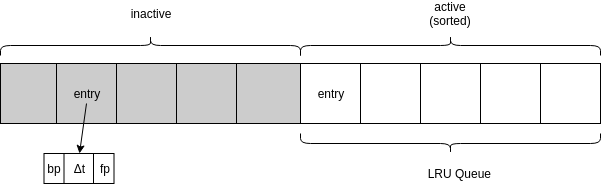
\includegraphics{figures/LRU-LC.png}
    \caption{Structure of LRU-LC}
    \label{fig:LRU-LC}
\end{figure}

\subsection{Clustering}
\subsubsection{CluStream Framework}



\section{Lossless Compression}
\subsection{LZ77}
\subsection{LZSS}
\subsection{A-LZSS}

\subsection{LEC}
\subsection{S-LEC}

\subsection{LZW}
\subsection{S-LZW}



\section{Lossy Compression}
